\section{实验内容\cite{pcl2002}}

\subsection{仪器与药品}

\ce{CCl4},二次去离子水,\SI{1000}{\milli\litre} 烧杯,\SI{250}{\milli\litre} 两口圆底烧瓶等。

WXI-04型压力-温度测定仪,SHB-III型循环水泵,电加热器,带电热套的磁力搅拌装置,冷凝水循环系统,真空缓冲罐,直形冷凝管,搅拌磁子,真空脂。

\subsection{实验步骤与条件}

\begin{figure}[H]
   \centering
   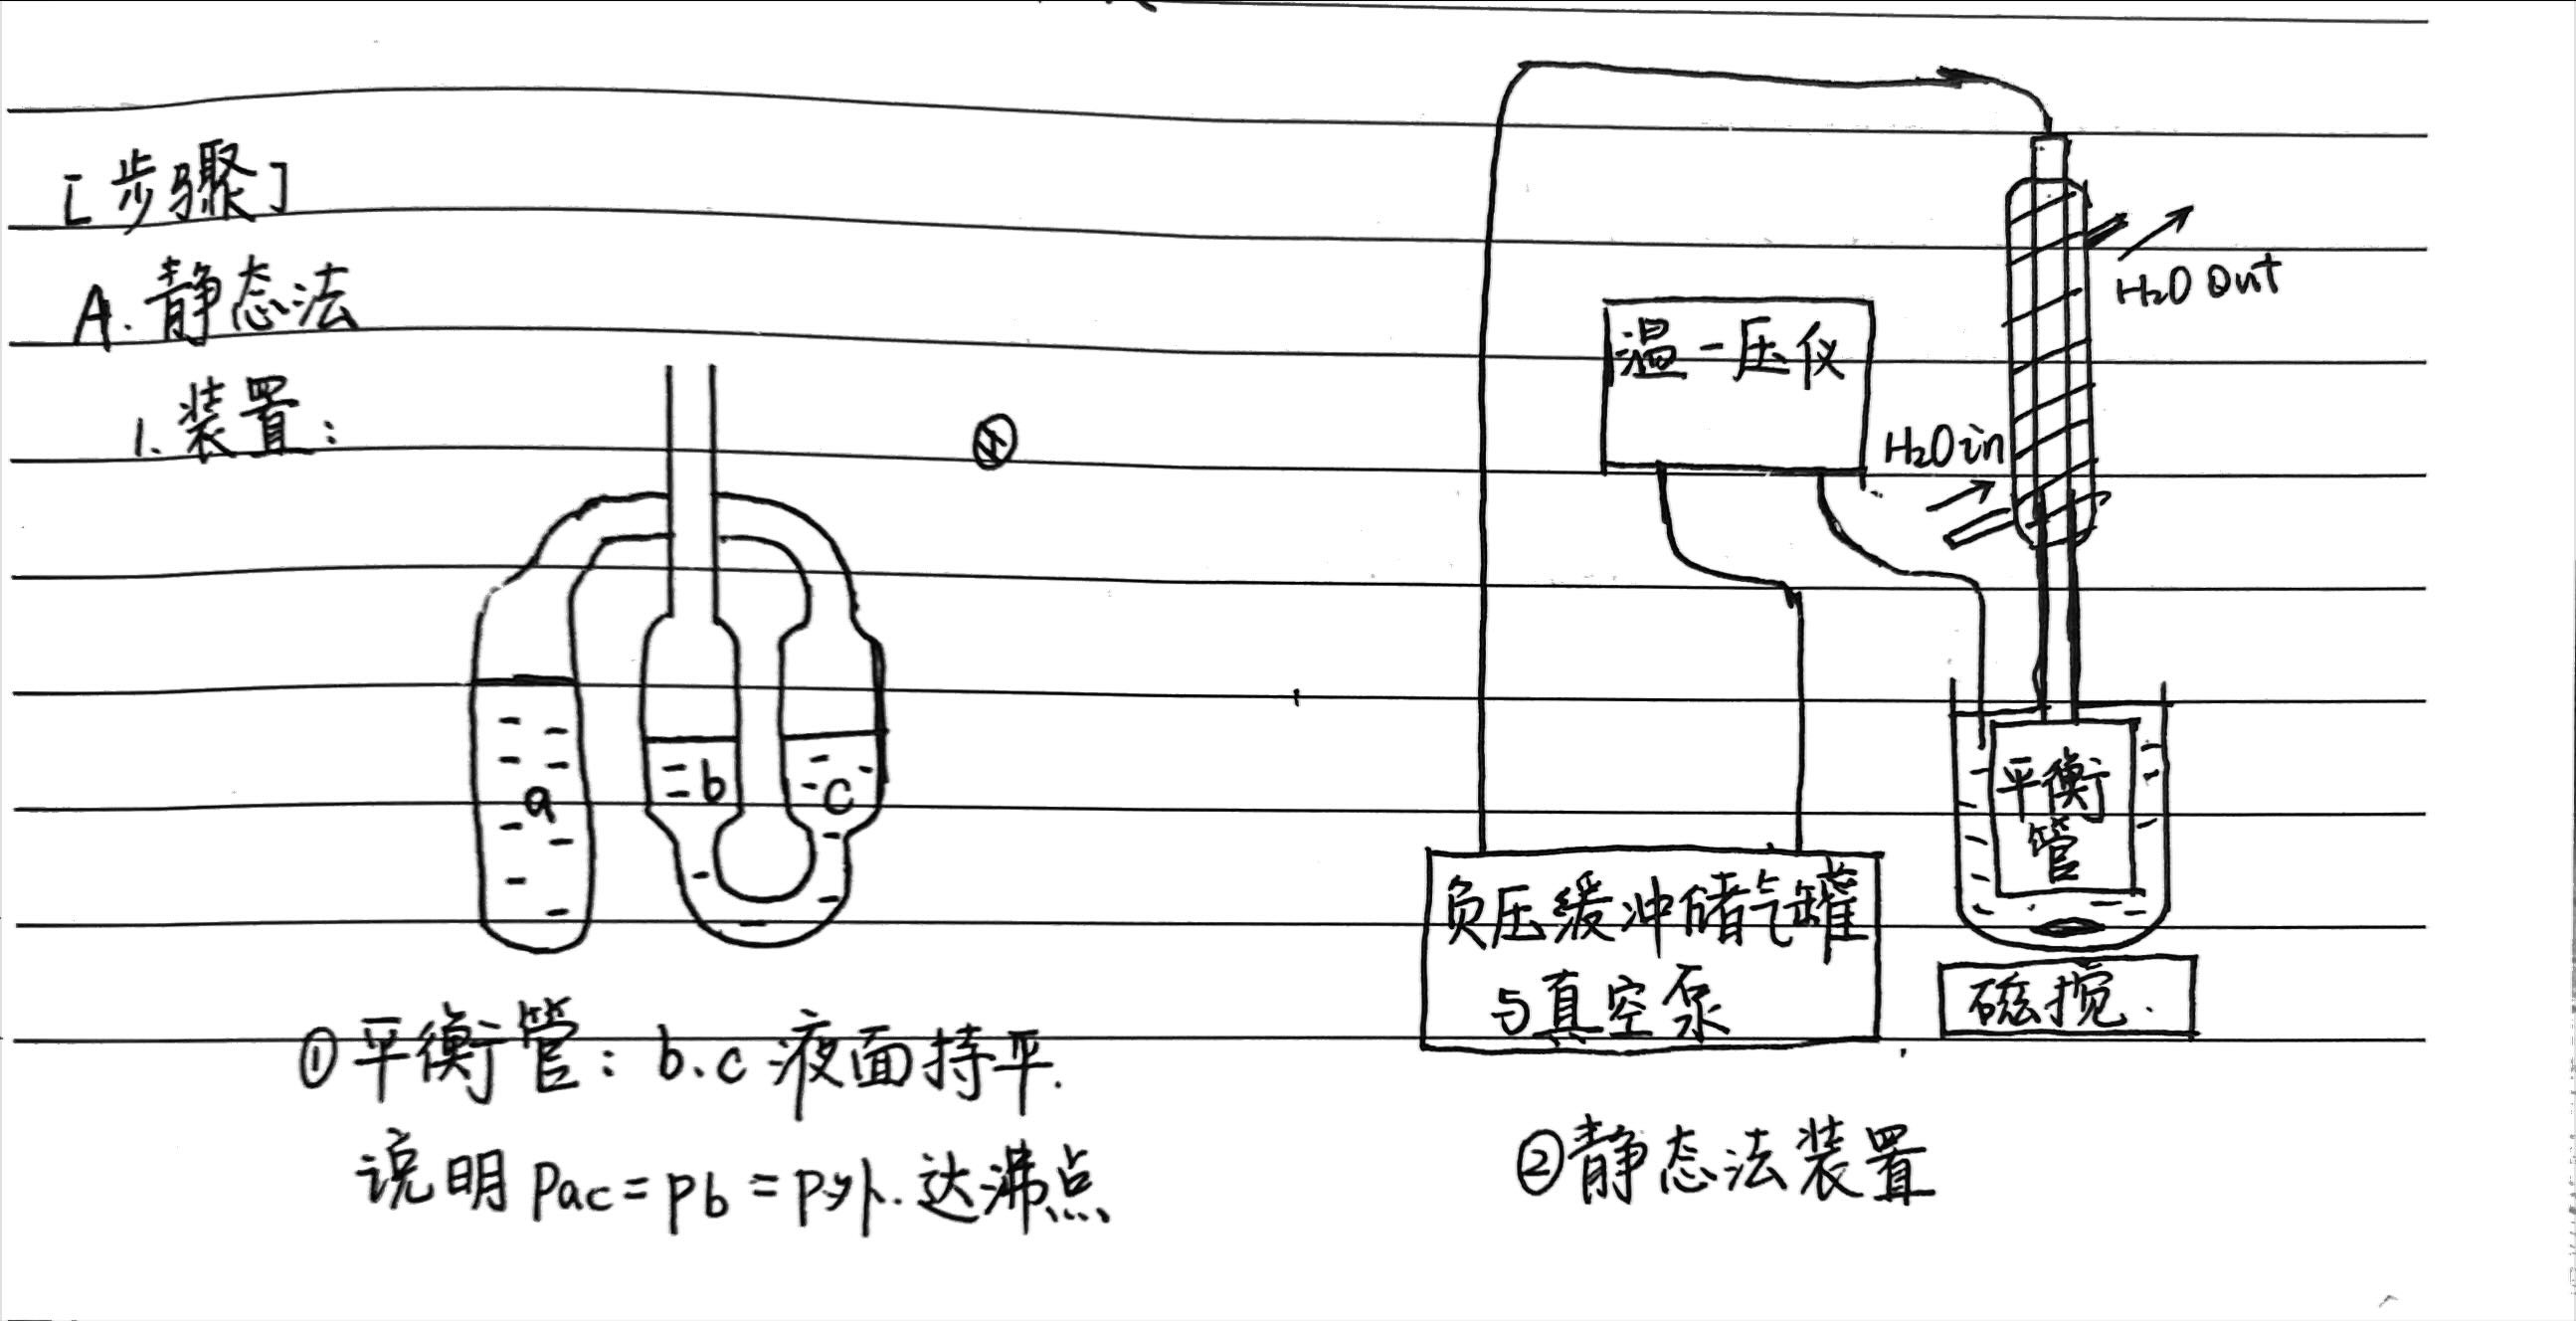
\includegraphics[width=.78\textwidth]{figures/0-3-1.jpg}
   \bicaption{实验仪器示意图}{Schematic Diagram of Experimental Apparatus}

\end{figure}

\subsection{静态法测 \ce{CCl4} 饱和蒸气压}
实验开始前,读取实验室内的大气压 \( p_0 = \SI{99.95}{kPa} \)。打开公用循环真空泵,旋转储气罐阀门,使系统与大气隔绝、与真空泵相通,使压力计示数降至 \( \SI{52.00}{kPa} \),记录温度为 \(\SI{20.67}{\celsius} \) ;密闭活塞使系统与真空原隔绝,\( \SI{3}{\minute} \) 后压力计示数为 \( \SI{52.03}{kPa} \),记录温度为 \(\SI{20.70}{\celsius} \),表明体系气密性符合要求。

使体系与大气相通,水浴加热至 \( \sim \SI{80}{\celsius} \),平衡管中有气泡产生,将平衡管中的空气排净。停止加热,不断搅拌,温度下降至一定程度时,\( b \) 管中气泡开始消失,\( c \) 管液面开始上升,同时 \( b \) 管液面下降。两管液面达到同一水平时,立即记下此时的温度计示数 \( t_b \) 和压力计示数 \( p^\prime \),重复赶气,平行测量多次 \ce{CCl4} 大气压下的沸点,直至结果一致。

立即关闭储气罐通向大气的活塞,先打开真空泉,再打开通真空泉的阀,使体系减压 \( \sim \SI{5}{kPa} \),液体重又沸腾。关闭通真空泉的阀,不断搅拌,冷却至 \( b \)、\( c \) 两管液面等高时,按下温度-压力测定仪上的绿色按钮,记录温度 \( t_b \) 和压力计示数 \( p^\prime \)。继续实验,每次减压 \( \sim \SI{5}{kPa} \),直至压差值为 \( \sim \SI{50}{kPa} \) 时,停止实验。

实验结束后, 读取实验室内的大气压 \( p_0 = \SI{99.90}{kPa} \), 取实验前后大气压的平均值 \( p_0 = \SI{99.92}{kPa} \) 作为实验过程中的大气压值。

\subsection{动态法测 \ce{H2O} 饱和蒸气压}

实验开始前,读取实验室内的大气压 \( p_0 = \SI{99.88}{kPa} \)。组装测量系统。将装有约 \SI{200}{\milli\litre} 去离子水和搅拌磁子的两口圆底烧瓶置于电加热套上并与冷凝管相连接。将温度探头通过橡皮塞插入烧瓶的侧口,探头尖端位于液面上侧,磨口处涂抹真空脂以防止漏气。打开回流冷凝水,调节流量适中。旋转储气罐阀门使系统与大气相通。打开公用循环真空泵,旋转储气罐阀门,使系统与大气隔绝、与真空泵相通,使压力计示数降至 \( \SI{50.30}{kPa} \),记录温度为 \(\SI{21.42}{\celsius} \) ;密闭活塞使系统与真空原隔绝,\( \SI{3}{\minute} \) 后压力计示数为 \( \SI{50.41}{kPa} \),记录温度为 \(\SI{21.42}{\celsius} \),表明体系气密性符合要求。

保持压差值为 \( \sim \SI{50}{kPa} \),开始加热,不断搅拌。记录烧瓶中水沸腾、温度计示数不再上升时的温度 \( t_b \) 和压力计示数 \( p^\prime \)。停止加热, 略微开启缓冲罐通大气的阀门, 使少量空气进入系统, 使内外压差降低 \SI{5}{kPa}, 关闭活塞, 重新加热至沸腾, 记录 \( t_b \) 和 \( p^\prime \)。重复上述步骤, 直至系统与大气完全相通。继续加热, 测量 \ce{H2O} 大气压下的沸点。平行测量 3 次,每次等体系温度略微冷却、水不再沸腾后重新加热至沸腾后测量。

实验结束后, 读取实验室内的大气压 \( p_0 = \SI{99.84}{kPa} \), 取实验前后大气压的平均值 \( p_0 = \SI{99.86}{kPa} \) 作为实验过程中的大气压值。


